\chapter{Grundlagen}\label{chap:Grundlagen}
\section{Mittelwert}\label{sec:Grundlagen:Mittelwert}
Der Mittelwert, das Mittel oder auch der Durchschnitt entspricht nach \autoref{eq:Mittelwert} der Summe der einzelnen Werte $x_1$, $x_2$, $x_3$ ... $x_n$ geteilt durch ihre Anzahl $n$.
\begin{equation}\label{eq:Mittelwert}
    \bar x = \frac{1}{n}\sum_{i=1}^n x_i
\end{equation}

\section{Susceptible-Infectious-Removed-Modell}\label{sec:Grundlagen:SIR}
Ein Weg zur Beschreibung der Pandemie bietet das \glqq{}Susceptible-Infectious-Removed-Modell\grqq{} (SIR-Modell) \autocite{SIR}. Dieses Modell teilt die Mitglieder einer Menschengruppe in eine der drei folgenden Kategorien ein und ermöglicht es, die zeitliche Entwicklung einer Pandemie übersichtlich darzustellen:
\begin{itemize}
    \item \glqq{}Susceptible\grqq{}: Menschen, welche angesteckt werden können.
    \item \glqq{}Infectious\grqq{}: Infizierte Menschen, welche weitere Menschen anstecken können. Werden auch als \glqq{}die aktiven Fälle\grqq{} bezeichnet.
    \item \glqq{}Removed\grqq{}: Menschen, welche in die Kategorie \glqq{}Infectious\grqq{} fielen, nun keine weiteren Menschen mehr anstecken können und aus dem Infektionsgeschehen entfernt wurden,
    in diesem Fall Genesene und Verstorbene. 
\end{itemize}
In dem hier verwendeten SIR-Modell wird weder die Geburten- noch die Sterberate beachtet, die angenommen Bevölkerung bleibt durchgehend konstant.

Zudem wird angenommen, das jedes Individuum nur einmal infiziert werden kann und die Infektion die einzige Möglichkeit darstellt, von der Kategorie \glqq{}Susceptible\grqq{} in die Kategorie \glqq{}Removed\grqq{} zu wechseln.
Somit fällt die Zahl der Menschen in der Kategorie \glqq{}Susceptible\grqq{} monoton und die Zahl der Menschen in der Kategorie \glqq{}Removed\grqq{} steigt monoton an.

\section{Bevölkerungsdichte}
Die Bevölkerungsdichte eines Gebietes $\rho_{Gebiet}$ wird berechnet, indem die Anzahl der Einwohner im Gebiet $n_{Einwohner\ Gebiet}$ durch die Fläche des Gebiets $A_{Gebiet}$ geteilt wird:
\begin{equation}\label{eq:Bevölkerungsdichte}
    \rho_{Gebiet} = \frac{n_{Einwohner\  Gebiet}}{A_{Gebiet}}
\end{equation}
\section{7-Tages Inzidenz}\label{sec:Grundlagen:7-Tages Inzidenz}
Die 7-Tages Inzidenz $i_t$ wird für jeden Tag $t$ seit Beginn der Pandemie berechnet.
Zuerst wird von der akkumulierte Zahl der Fälle am gewählten Tag $f_t$ die akkumulierte Zahl der Fälle sieben Tage zuvor $f_{t-7}$ abgezogen, dies ergibt die neu hinzugekommenen Fälle innerhalb von sieben Tagen.

Schlussendlich wird diese Zahl durch die Anzahl der Bewohner des Gebiets $p_{Gebiet}$ geteilt und mit 100.000 multipliziert. Dies ergibt \autoref{eq:7-Tages_Inzidenz}.
\begin{equation}\label{eq:7-Tages_Inzidenz}
    i_t= \frac{f_t-f_{t-7}}{p_{Gebiet}}\cdot 100.000
\end{equation}

Die 7-Tages Inzidenz bietet sich im Vergleich zur täglichen Fallzahl aus mehreren Gründen als Kennzahl für die Verbreitung eines Virus in einem Gebiet an:

Wie in \autoref{fig:neue_Fälle_pro_Wochentag_Deutschland} klar zu sehen, werden an Wochenenden im Schnitt deutlich weniger neue Fälle registriert als an den anderen Wochentagen.
Daher werden immer sieben Tage in der 7-Tages Inzidenz zusammengefasst.
\begin{figure}[H]
    \centering
    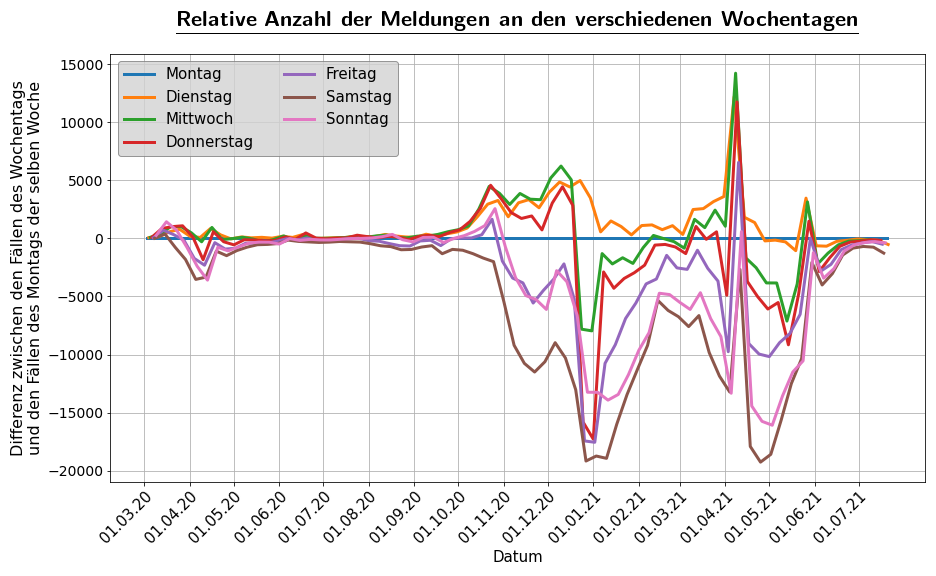
\includegraphics[width=0.95\textwidth]{figures/Grundlagen/neue_Fälle_pro_Wochentag_Deutschland.png}
    \caption{In Deutschland neu gemeldete COVID-19 Fälle am jeweiligen Wochentag im Vergleich zu den am Montag der selben Woche gemeldeten Fälle.}
    \label{fig:neue_Fälle_pro_Wochentag_Deutschland}
\end{figure}
Da die Bevölkerung der deutschen Landkreise und Regierungsbezirke nicht identisch ist, wird jeweils durch die Bevölkerungszahl geteilt, um die einzelnen Gebiete miteinander vergleichen zu können.

Aufgrund der ansonsten sehr kleinen Zahlen, bietet es sich zudem an, das Ergebnis mit 100.000 zu multiplizieren.

Dies sind die drei Begründungen für die drei Schritte in der Berechnung der 7-Tages Inzidenz nach \autoref{eq:7-Tages_Inzidenz}.


\section{Korrelationsanalyse mithilfe einer Faltung}\label{sec:BeschreibungKorrelationsanalyse}

\subsection{Berechnung der Korrelationswerte}\label{sec:Grundlagen:BerechnungderKorrelationwertes}
Um festzustellen, ob die 7-Tages Inzidenzen einiger Landkreise im Vergleich zu anderen Landkreisen eher voraus- oder nacheilen, wird die Korrelationsfunktion verwendet \autocite{Korrelation}.

Bei diskreten Werten, aufgeteilt in zwei Zeitserien $X$ und $Y$, wie in diesem Fall, basiert die Korrelationsanalyse auf einer diskreten Faltung:
Für eine zeitliche Verschiebung $\tau$ wird mit jedem Wert $x_i$ zum jeweiligen Zeitpunkt $t_i$ aus der ersten Zeitserie mit dem zugehörigen Wert $y_i$ aus der zweiten Zeitserie ein Produkt gebildet. Der zugehörige Wert aus der zweiten Zeitserie entspricht hierbei dem Zeitpunkt $t$ des Wertes der ersten Zeitserie plus die gewählte Verschiebung $\tau$. Sollte dieser zweite Wert nicht existieren, wird kein Produkt gebildet.

Für jede zeitliche Verschiebung $\tau$, für die mindestens ein Produkt gebildet wird, werden alle möglichen Produkte aufsummiert.

Somit ergibt sich \autoref{eq:Korrelation}, mit $n := $ Länge von $X$ und wenn $y_{i+\tau} \not\in Y$, dann $y_{i+\tau} := 0$:
\begin{equation}\label{eq:Korrelation}
    c(\tau) = \sum_{i=1}^n x_i\cdot y_{i+\tau}
\end{equation}


Bildlich gesprochen wird die zweite Zeitserie an der ersten Zeitserie vorbeigeschoben, beginnend an dem Punkt, an dem ausschließlich das erste Element der ersten Zeitserie mit dem letzten Element der zweiten Zeitserie multipliziert wird. Dies ist beispielhaft mit den Folgen $[1,2,3,2]$ und $[5,7,5,1]$ in \autoref{fig:Korrelation Beispiel} dargestellt.

\begin{figure}[H]
    \centering
    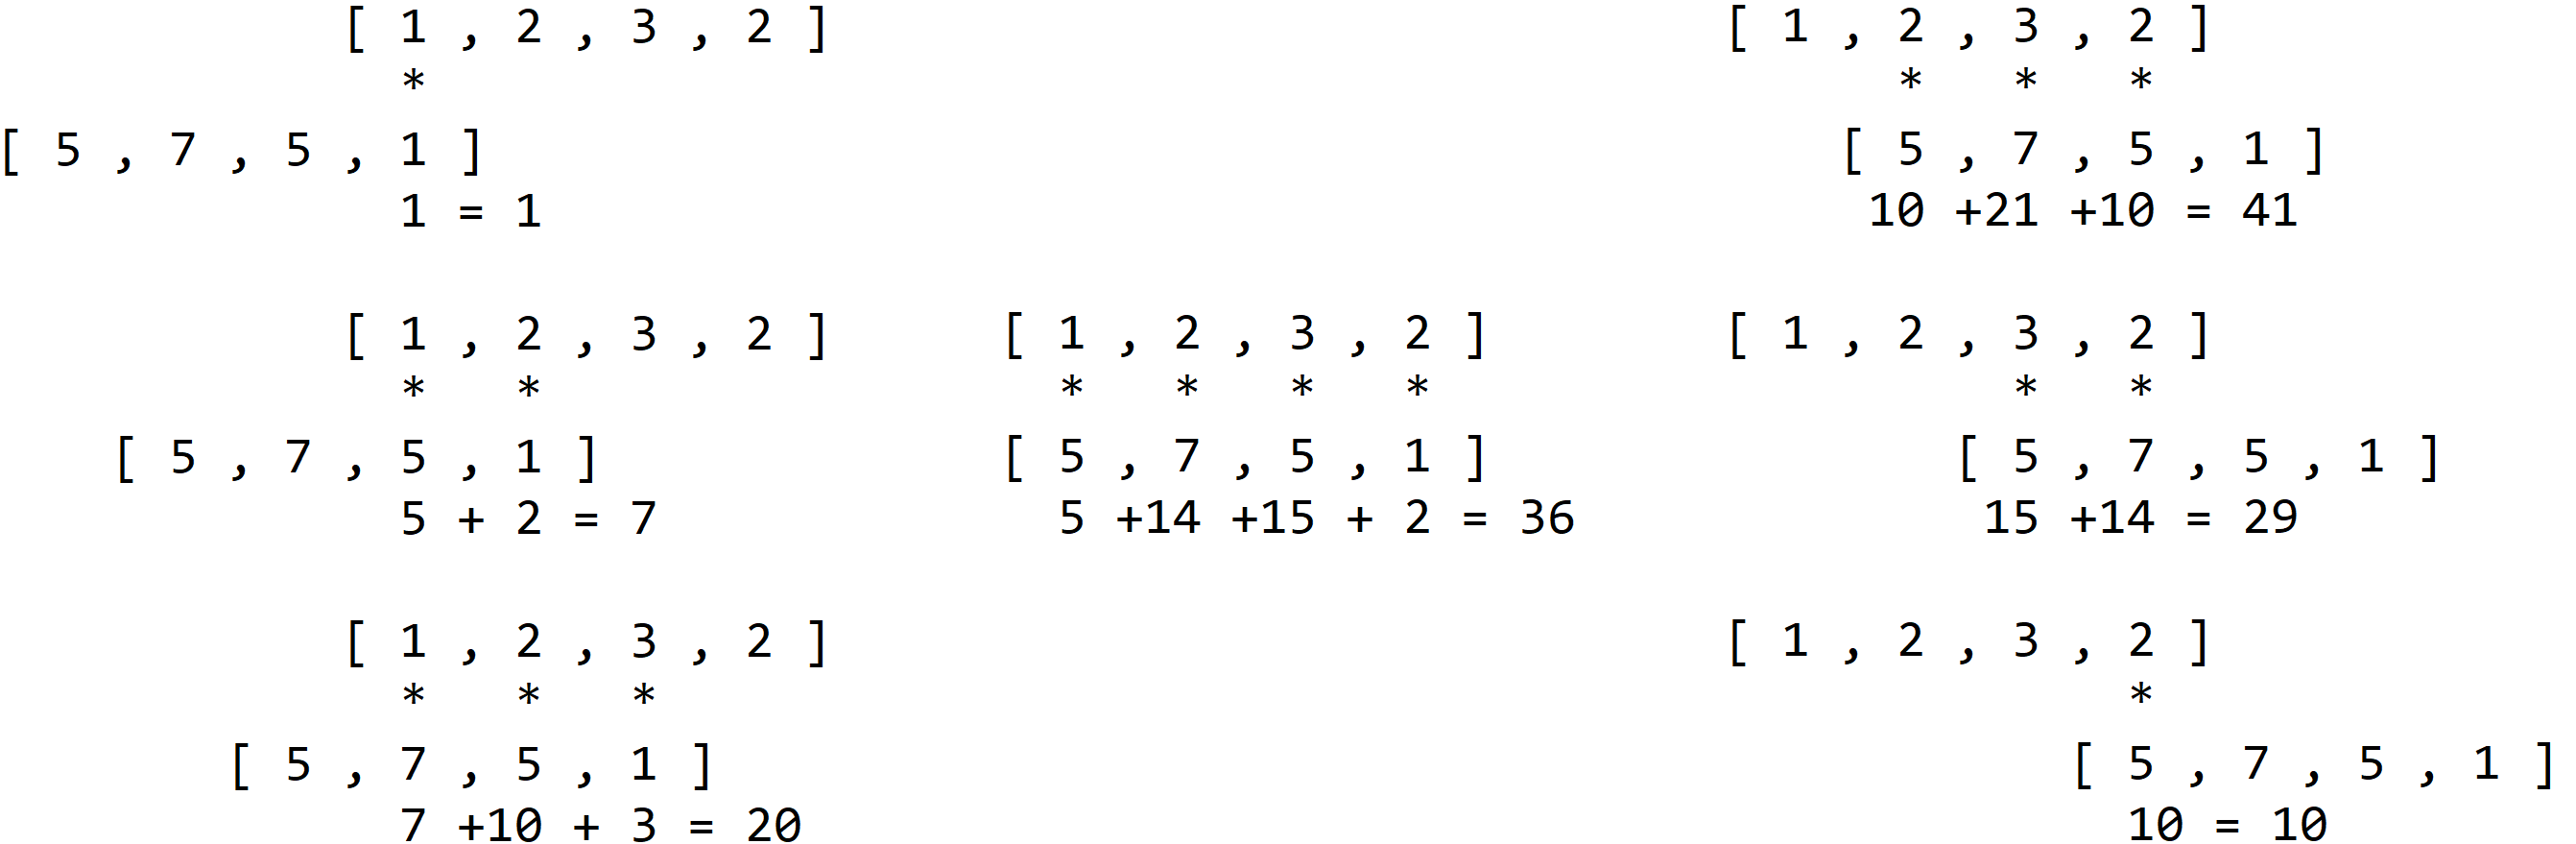
\includegraphics[width=\textwidth]{figures/Grundlagen/Korrelation.png}
    \caption{Beispielhafte Darstellung einer Faltung anhand der Folgen $[1,2,3,2]$ und $[5,7,5,1]$. Auf der linken Seite hinter dem Gleichheitszeichen von oben nach unten die Korrelationswahrscheinlichkeiten für die negativen Verschiebungen $\tau=-3$, $\tau=-2$ und $\tau=-1$. Entsprechend in der Mitte bei keine Verschiebung ($\tau=0$) und rechts für die positiven Verschiebungen $\tau=1$, $\tau=2$ und $\tau=3$}
    \label{fig:Korrelation Beispiel}
\end{figure}

Da bei einer Korrelationsanalyse nach \autoref{eq:Korrelation} Summen aus mehr Produkten übergewichtet werden und Zeitserien mit größeren Werten größere Korrelationswerte erzeugen, müssen die Korrelationswerte noch skaliert werden.

Um zum einen die unterschiedliche Anzahl der Produkte auszugleichen, werden die Summen durch die Anzahl ihrer Summanden geteilt, wie in \autoref{eq:skalierte_Korrelation_geteilt_durch_Produkte} gezeigt. Ohne diese Gewichtung würden zwei Zeitserien mit konstanten Werten größer null bei einer Verschiebung $\tau=0$ die größte Korrelation aufweisen und die Korrelation bei betragsmäßig größeren Verschiebungen abnehmen, was nicht gewünscht ist.

Da jede Zeitserie die gleiche Länge $n$ hat, erhält man die Anzahl der Summanden indem man
den Betrag der Verschiebung $\vert\tau\vert$
von der Länge der Zeitserie $n$ abzieht:

\begin{equation}\label{eq:skalierte_Korrelation_geteilt_durch_Produkte}
    c(\tau) =\frac{1}{n-\vert\tau\vert} \sum_{i=1}^n x_i\cdot y_{i+\tau}
\end{equation}

Um zum anderen die tendenziell größeren Werte mancher Zeitserien auszugleichen, werden die Werte aller Zeitserien mithilfe des sogenannten \glqq{}Autokorrelationswerts für die Verschiebung $\tau=0$\grqq{} gewichtet: Er beschreibt den Wert der Korrelation einer Zeitserie mit sich selbst bei keiner zeitlichen Verschiebung. Wie in \autoref{eq:skalierte_Korrelation} zu sehen, werden die Werte einer Zeitserie gewichtet, indem sie durch die Wurzel des Autokorrelationswerts für die Verschiebung $\tau=0$ dieser Zeitserie geteilt werden.

\begin{equation}\label{eq:skalierte_Korrelation}
    c(\tau) =
    \frac{1}{n-\vert\tau\vert}
    \sum_{i=1}^n
    \frac{x_i}{\sqrt{\frac{1}{n}\sum_{i=1}^n x_i^2}}
    \cdot
    \frac{y_{i+\tau}}{\sqrt{\frac{1}{n}\sum_{i=1}^n y_i^2}}
    =
    \frac{n}{n-\vert\tau\vert}
    \frac{\sum_{i=1}^n x_i \cdot y_{i+\tau}}
    {\sqrt{\sum_{i=1}^n x_i^2}
    \sqrt{\sum_{i=1}^n y_i^2}}
\end{equation}


Zudem wird von jedem Wert der Zeitserie $x_i$ der Mittelwert $\overline x = \frac{1}{n}\sum_{i=1}^n x_i$ abgezogen, dadurch lassen sich Antikorrelationen feststellen: Wenn beispielsweise die Anzahl der COVID-19 Infektionen eines Landkreises zu einem Zeitpunkt überdurchschnittlich wächst, also die 7-Tages-Inzidenz minus dem Mittelwert der 7-Tages-Inzidenzen positiv ist, und das andere Edukt aus der anderen Zeitserie negativ ist, also in dem anderen Landkreis die Anzahl der COVID-19 Infektionen unterdurchschnittlich wächst, ergibt sich ein negatives Produkt, da sich die Situation in dem einen Landkreis  schneller als üblich verschlechtert, während sich die Situation im anderen Landkreis verbessert oder langsamer als üblich verschlechtert.

Ergibt die Summe aus all den Produkten einer Korrelation eine negative Zahl, scheint die 7-Tages Inzidenz des einen Landkreises zu fallen oder langsam zu steigen, während die 7-Tages Inzidenz des anderen Landkreises steigt oder langsam fällt, dies wird hier Antikorrelation genannt.

Mit allen Ergänzungen berechnet sich die Korrelation $c(\tau)$ zwischen Zeitserie $X:|X|=n$ mit den Werten $x_i\in X$ und Zeitserie $Y:|Y|=n$ mit den Werten $y_i \in Y$ und einer Verschiebung $\tau$ relativ zu $X$ mithilfe der Mittelwerte der Zeitserien $\overline x,\ \overline y$ wie in \autoref{eq:komplette_skalierte_Korrelation} beschrieben.
\begin{equation}\label{eq:komplette_skalierte_Korrelation}
    c(\tau) =\frac{n}{n-\vert\tau\vert}
    \frac{\sum_{i=1}^n (x_i-\overline x)\cdot (y_{i+\tau}-\overline y)}{\sqrt{\sum_{i=1}^n (x_i-\overline x)^2}\sqrt{\sum_{i=1}^n (y_i-\overline y)^2}}
\end{equation}

\subsection{Korrelation zwischen zwei Gebieten am Beispiel von Flensburg und Kiel}
Um die verwendete Terminologie und die hergeleiteten Gleichungen anhand eines Beispiels näher zu bringen, werden in diesem Abschnitt die einzelnen Schritten einer Korrelationsanalyse ausgeführt. Als Beispiel dient hierfür die Korrelation zwischen den 7-Tages Inzidenzen der Stadtkreise Flensburg und Kiel. Die 7-Tages Inzidenzen sind in \autoref{fig:Inzidenz_Flensburg} und \autoref{fig:Inzidenz_Kiel} abgebildet, jeweils einmal im Original und einmal um die mittlere 7-Tages Inzidenz in x-Richtung nach unten verschoben.

\begin{figure}[H]
    \centering
    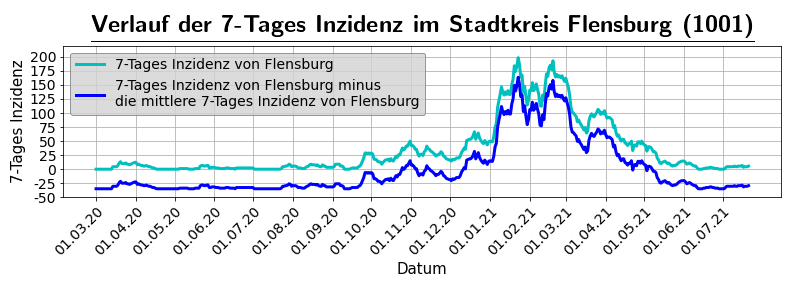
\includegraphics[width=0.95\textwidth]{figures/Grundlagen/Inzidenz_Flensburg.png}
    \caption{Der Verlauf der 7-Tages Inzidenz des Stadtkreises Flensburg (Gemeindeschlüssel 1001).
    In Hellblau sind ist der originale Verlauf der 7-Tages Inzidenz dargestellt. Der Verlauf der 7-Tages Inzidenzen, von denen der Mittelwert der 7-Tages Inzidenzen von Flensburg abgezogen wurde, ist blau dargestellt.}
    \label{fig:Inzidenz_Flensburg}
\end{figure}
\begin{figure}[H]
    \centering
    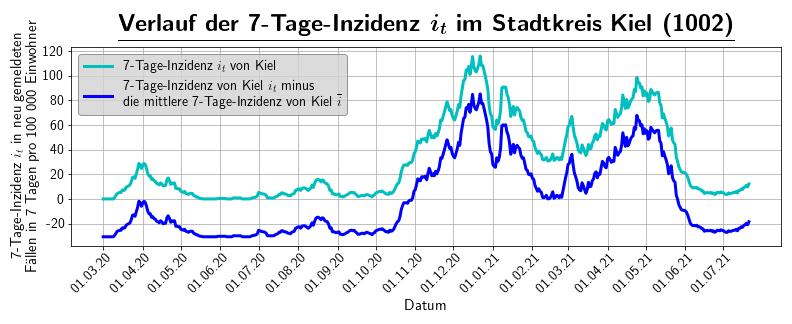
\includegraphics[width=0.95\textwidth]{figures/Grundlagen/Inzidenz_Kiel.png}
    \caption{Der Verlauf der 7-Tages Inzidenz des Stadtkreises Kiel (Gemeindeschlüssel 1002).
    In Hellblau sind ist der originale Verlauf der 7-Tages Inzidenz dargestellt. Der Verlauf der 7-Tages Inzidenzen, von denen der Mittelwert der 7-Tages Inzidenzen von Kiel abgezogen wurde, ist blau dargestellt.}
    \label{fig:Inzidenz_Kiel}
\end{figure}
In \autoref{fig:correlation_Flensburg_Kiel} ist die diskrete Faltung abgebildet, wie sie der Korrelationsanalyse zugrunde liegt und in \autoref{eq:Korrelation} definiert ist.
\begin{figure}[H]
    \centering
    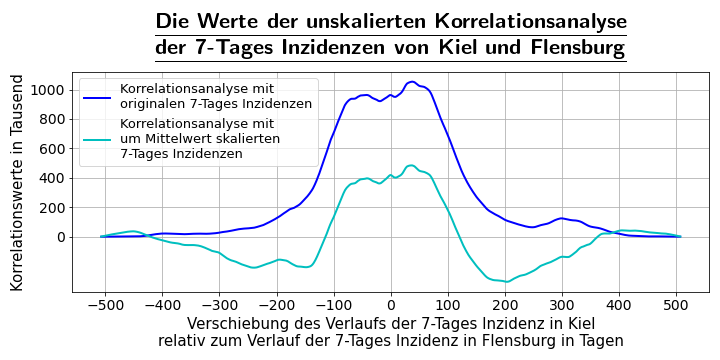
\includegraphics[width=0.95\textwidth]{figures/Grundlagen/correlation_Flensburg_Kiel.png}
    \caption{Ergebnis der diskreten Faltung der 7-Tages Inzidenzen der Stadtkreise Kiel und Flensburg.
    In Hellblau ist das Ergebnis der Faltung mit den originalen 7-Tages Inzidenzen dargestellt. Das Ergebnis der Faltung mit den 7-Tages Inzidenzen, von denen der Mittelwert der 7-Tages Inzidenzen des jeweiligen Landkreises abgezogen wurde, ist blau dargestellt.}
    \label{fig:correlation_Flensburg_Kiel}
\end{figure}
\autoref{fig:correlation_Flensburg_Kiel_scaled_autocorrelation} ergibt sich, wenn die Summen jeweils durch die Anzahl ihrer Summanden (den Produkten) geteilt werden, wie in \autoref{eq:skalierte_Korrelation_geteilt_durch_Produkte} beschrieben. Klar zu erkennen die verstärkten Ausschläge am linken und rechten Rand.
\begin{figure}[H]
    \centering
    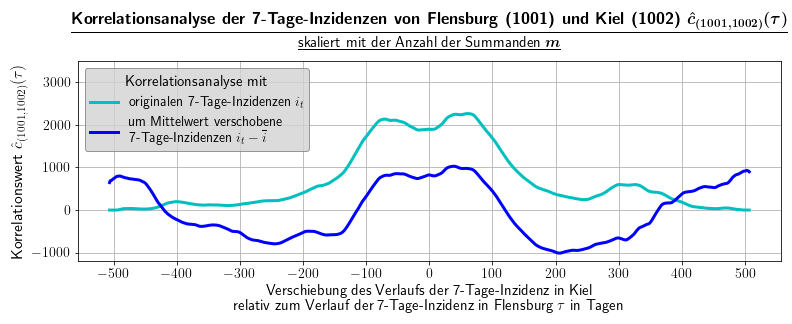
\includegraphics[width=0.95\textwidth]{figures/Grundlagen/correlation_Flensburg_Kiel_scaled_autocorrelation.png}
    \caption{Korrelationsanalyse der 7-Tages Inzidenzen der Stadtkreise Kiel und Flensburg ohne Skalierung mithilfe der Autokorrelation.
    In Hellblau ist das Ergebnis der Korrelationsanalyse mit den originalen 7-Tages Inzidenzen dargestellt. Das Ergebnis der Korrelationsanalyse mit den 7-Tages Inzidenzen, von denen der Mittelwert der 7-Tages Inzidenzen des jeweiligen Landkreises abgezogen wurde, ist blau dargestellt.}
    \label{fig:correlation_Flensburg_Kiel_scaled_autocorrelation}
\end{figure}
In \autoref{fig:correlation_Flensburg_Kiel_scaled_autocorrelation} sind die Ergebnisse der kompletten Korrelationsanalyse abgebildet, wie sie mithilfe von \autoref{eq:skalierte_Korrelation} erzeugt werden.
\begin{figure}[H]
    \centering
    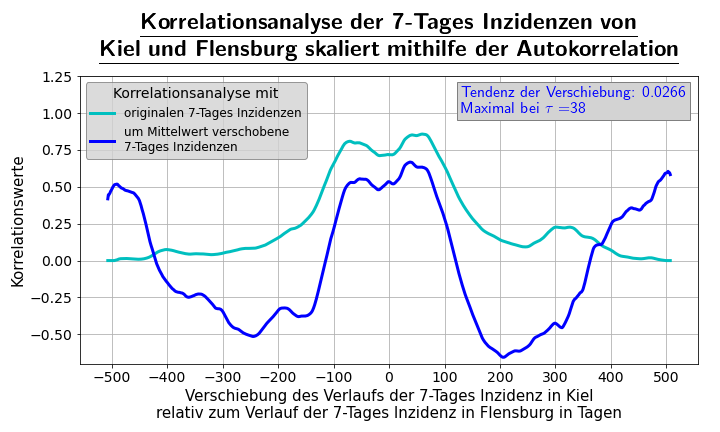
\includegraphics[width=0.95\textwidth]{figures/Grundlagen/correlation_Flensburg_Kiel_scaled_complete.png}
    \caption{Vollständige Korrelationsanalyse der 7-Tages Inzidenzen der Stadtkreise Kiel und Flensburg skaliert mithilfe der Autokorrelation.
    In Hellblau ist das Ergebnis der Korrelationsanalyse mit den originalen 7-Tages Inzidenzen dargestellt. Das Ergebnis der Korrelationsanalyse mit den 7-Tages Inzidenzen, von denen der Mittelwert der 7-Tages Inzidenzen des jeweiligen Landkreises abgezogen wurde, ist blau dargestellt.}
    \label{fig:correlation_Flensburg_Kiel_scaled_complete}
\end{figure}

In \autoref{fig:correlation_Flensburg_Kiel_scaled_complete} ist schön zu erkennen, das die Korrelationsanalyse von zwei Zeitserien mit 508 7-Tages Inzidenzen 1015 Korrelationswerte ergibt.
Für jeden der 412 Landkreis ergeben sich daher aus der Korrelationsanalyse mit sich selbst und jedem anderen Landkreise 418.180 Werte, ebenso ergeben sich für jeden der 38 Regierungsbezirk 38.570. Dies ergibt in Summe $
%38.570\cdot 38 + 418.180\cdot412 =
1.465.660+172.290.160=173.755.820$ Werte.

Jeder Wert gibt die Wahrscheinlichkeit einer Korrelation bei der jeweiligen Verschiebung an, wobei die zugeordneten Verschiebungen von links nach rechts bei jedem Schritt um eins zunehmen und der mittlerste der Korrelationswerte der Verschiebung $\tau = 0$ zugeordnet ist. Die Verschiebung ist im Kontext dieser Arbeit stets in ganzen Tagen zwischen $-507$ und $507$ angegeben. Der Wert an Position 501 in der Liste der Korrelationswerte gibt also an, wie wahrscheinlich der Verlauf der 7-Tages Inzidenz des ersten Gebiets mit dem um eine Woche nach links verschobenen Verlauf der 7-Tages Inzidenz des zweiten Gebiets korreliert.

\subsection{Komprimierung und Darstellung als Matrizen}\label{sec:Grundlagen:Korrelation:Komprimierung}
Das Ziel der nachfolgend beschriebenen Schritte ist, die Korrelationswerte eines Gebiets auf einen Wert zusammenzuführen, sodass man einfach und schnell auffallende Korrelationen zwischen zwei oder mehreren Gebieten finden kann.

In dieser Arbeit werden nur Korrelationen mit einem zeitlichen Versatz zwischen $\tau=-50$ und $\tau=50$ betrachtet, da zum einen eine Interpretation für eine Verschiebung von mehr als 4 Wochen sehr schwierig ist und zum anderen einzelne Ausreißer bei größeren Verschiebungen stärker ins Gewicht fallen, weil immer weniger Produkte aufsummiert werden. Dies fällt auch in \autoref{fig:correlation_Flensburg_Kiel_scaled_autocorrelation} im Vergleich zu \autoref{fig:correlation_Flensburg_Kiel} an den Rändern der Graphen auf.

Um ein detailliertes Bild zu erhalten, werden zudem Korrelationsanalysen für die Verschiebungen $\tau\in[-30,30]$ und $\tau\in[-14,14]$ durchgeführt.

Somit sind jeder Kombination aus zwei Landkreisen nur noch höchstens 101 Werte zugeordnet. Diese Werte werden in zwei verschiedenen Varianten zu einem Wert zusammengefasst:
\begin{itemize}
    \item Die Verschiebung mit dem maximalen Korrelationswert: Die zeitliche Verschiebung, bei der die Korrelationsanalyse den größten Wert angibt. Sie sagt aus bei welcher Verschiebung in Tagen am wahrscheinlichsten eine Korrelation vorliegt.
    \item Die Tendenz der Verschiebung: 
    Das Mittel der Differenz zwischen den Werten der betragsmäßig gleichen Verschiebungen.
    Das Resultat ermöglicht eine grobe Einschätzung, ob der maximale Wert nur ein Ausreißer ist oder nicht.
\end{itemize}

Die Berechnung der Tendenz der Verschiebung ist etwas komplexer und wird daher ebenfalls am Beispiel der Korrelationsanalyse der Stadtkreise Kiel und Flensburg erklärt.
In \autoref{fig:Flensburg_Kiel_Verschiebung_Tendenz} ist die Berechnung graphisch dargestellt.
Die Tendenz der Verschiebung berechnet sich aus der Liste der Korrelationswerte $C:\vert C\vert =m$, genauer gesagt aus ihrer Länge $m$ und ihren Werten $c_\tau$,$ -\lfloor m/2 \rfloor\geq \tau\leq \lfloor m/2 \rfloor$:
\begin{equation}
    s_{Tendenz} = \frac{1}{\lfloor m/2 \rfloor}
    \sum_{\tau=1}^{\lfloor m/2 \rfloor}c_{\tau}-c_{-\tau}
\end{equation}
In \autoref{fig:Flensburg_Kiel_Verschiebung_Tendenz} entspricht der blaue Graph den Werten der Korrelationsanalyse, wie sie auch in \autoref{fig:correlation_Flensburg_Kiel_scaled_complete} abgebildet sind. Um bildlich die Differenz zwischen den Werten der betragsmäßig gleichen Verschiebungen darzustellen, werden die Werte der negativen Verschiebungen an der Vertikalen bei $x=0$ gespiegelt und Lila eingefärbt.

Da die Linke Seite gespiegelt wird, ist sie nicht weiter von Bedeutung. In den Zwischenräumen der beiden Graphen und auf der Horizontalen bei $y=0$ sind die Differenzen der Werte der betragsmäßig gleichen Verschiebungen aufgezeichnet, deren Mittel der Tendenz der Verschiebung entspricht. Diese ist als dunkelblaue Horizontale bei $y=0.0266$ dargestellt.

\begin{figure}[H]
    \centering
    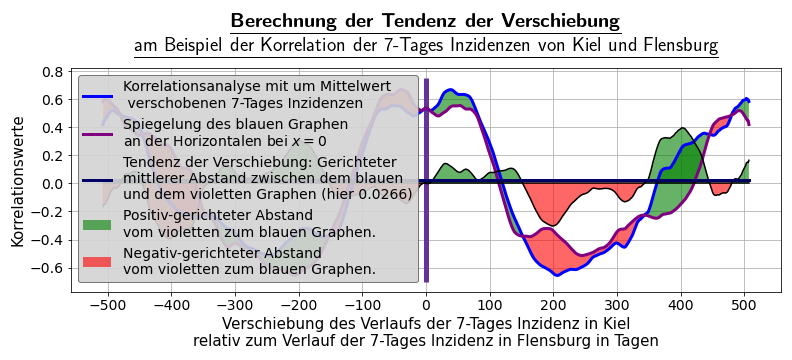
\includegraphics[width=0.95\textwidth]{figures/Grundlagen/correlation_Flensburg_Kiel_Verschiebung_Tendenz.png}
    \caption{Graphische Darstellung der Berechnung der Tendenz der Verschiebung.}
    \label{fig:Flensburg_Kiel_Verschiebung_Tendenz}
\end{figure}

Somit lässt sich zum einen die Verschiebung mit dem maximalen Korrelationswert ermitteln und einfach interpretieren.
Da hierfür jedoch nur ein Wert herausgenommen wird, bietet es sich zum anderen an, die Tendenz der Verschiebung zu berechnen und mit der Verschiebung mit dem maximalen Korrelationswert zu vergleichen.



Um dies für alle Landkreise und Regierungsbezirke zu ermöglichen, werden die beiden Werte jeweils in einer Matrix dargestellt: Jeder Zeile und Spalte wird der Index für ein Gebiet zugeordnet. In die Zellen werden entweder die Verschiebungen mit dem maximalen Korrelationswert oder die Tendenzen der Verschiebung eingetragen. Ein spezifischer Wert in einer Zelle stammt aus der Korrelationsanalyse der Gebiete, die der Zeile und der Spalte zugeordnet sind.
Die Matrizen sind (mit verkehrtem Vorzeichen) symmetrisch an der Diagonalen von links oben nach rechts unten. Die Diagonalen sind mit Nullen besetzt, da die Werte der positiven Verschiebung symmetrisch zu den Werten der negativen Verschiebung sind und die Korrelation mit sich selbst trivialerweise bei einer Verschiebung von $\tau=0$ am größten ist, da die Werte und Trends komplett identisch sind.

Um den Gebieten selbst Werte zuzuordnen und nicht nur in Kombination mit einem anderen Gebiet, wird sowohl bei den Maximalwerten wie auch den Tendenzen der Verschiebung der Mittelwert gebildet, indem die Zeilen der Matrizen aufsummiert werden und durch die Anzahl der Spalten geteilt werden.
\section{Farbgebung}\label{sec:Grundlagen:Farbgebung}
Um schnell verständliche Abbildungen bereitstellen zu können, werden die Werte skaliert und die Farbgebung der Deutschlandkarten derart angepasst, dass das gesamte Farbspektrum abgedeckt wird. Das Farbspektrum reicht gemäß den Farben des Regenbogens von blau über grün zu gelb zu rot, wie in \autoref{fig:color_schemes} demonstriert. Die niedrigsten Werte werden blau gefärbt.
Da manche dieser Farbwerte im Kontrast zu einem weißen Hintergrund schwer zu erkennen sind, ist der Hintergrund der meisten Abbildungen grau.

\begin{figure}
    \centering
    
\includegraphics[width=0.8\textwidth]{figures/Grundlagen/color_schemes.png}
    \caption{Das Farbspektrum, in welchem sich die Darstellungen bewegen. Von links nach rechts steigen die eingegebenen Werte konstant. Der angegebene Wert wird jeweils anhand des ersten und des letzten Werten einer Referenzliste linear in diesem Spektrum verortet.}
    \label{fig:color_schemes}
\end{figure}

Die Matrizen werden durch die verwendete Programmbibliothek \glqq{}Matplotlib\grqq{} automatisch eingefärbt.